\documentclass[mathserif]{beamer}

\usepackage{beamerthemesplit} % TODO: use different beamer theme
\usepackage{framed}

\title{SIAM: Getting Started with \LaTeX}
\author{Matthew Michelotti}
\date{\today}

\renewcommand{\arraystretch}{1.1}

\begin{document}

\frame{\titlepage}

\begin{frame}[fragile]
  \frametitle{What is \LaTeX{}?}

  \begin{itemize}
  \item \LaTeX{} is a high-quality typesetting system
  \item \LaTeX{} markup is converted into nice looking pdf files
  \end{itemize}

  \begin{minipage}{.38\textwidth}
  \begin{framed}
    \tiny
    \begin{verbatim}\documentclass[12pt]{article}
\usepackage{amsmath}
\title{\LaTeX}
\date{}
\begin{document}
  \maketitle
  \LaTeX{} is a document
  preparation system for the
  \TeX{} typesetting program.
  It offers programmable desktop
  publishing features and
  ...
  \begin{align}
    E &= mc^2 \\
    m &= \frac{m_0}
      {\sqrt{1-\frac{v^2}{c^2}}}
  \end{align}
\end{document}\end{verbatim}
  \end{framed}
  \end{minipage}
  $\rightarrow$
  \begin{minipage}{.55\textwidth} 
  \begin{framed}
    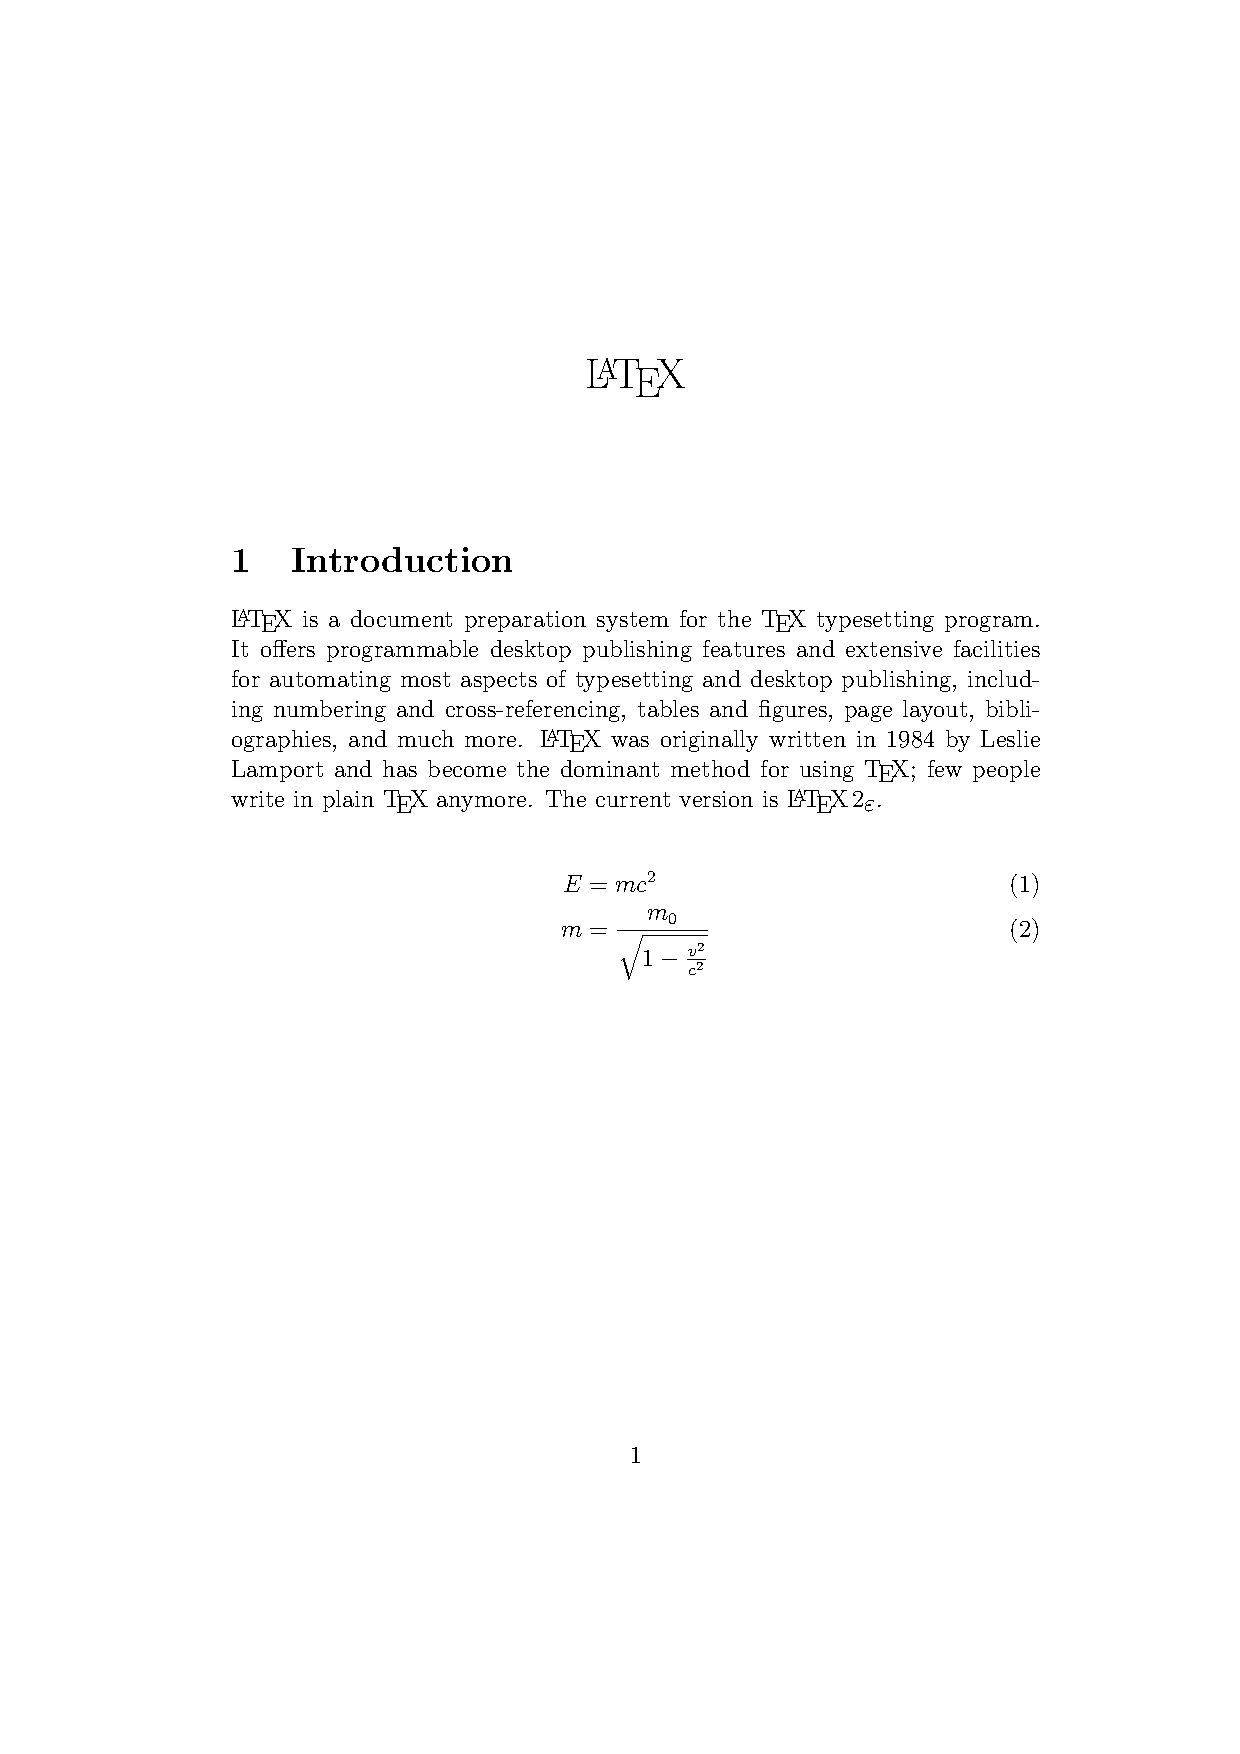
\includegraphics[trim = 33mm 127mm 33mm 59mm, clip, width=\textwidth]{figures/example_article.pdf}
  \end{framed}
  \end{minipage}
\end{frame}

\begin{frame}[fragile]
  \frametitle{Why Use \LaTeX{}?}
  \begin{itemize}
    \item Produces high-quality documents
    \item Offers precise control over how document looks
    \item Excellent for typesetting mathematics
    \item Automated references, citations, etc.
    \item Widely used for academic journals
    \item Free
    \item Multi-platform
  \end{itemize}
\end{frame}

\frame{
  \frametitle{Exercise 1: Compiling}
  \begin{itemize}
    \item Go to website www.compileonline.com/try\_latex\_online.php
    \item Compile the example \LaTeX{} file on this website
    \begin{itemize} \item The result should look as follows: \end{itemize}
  \end{itemize}

  \centerline{
  \begin{minipage}{.6\textwidth} 
  \begin{framed}
    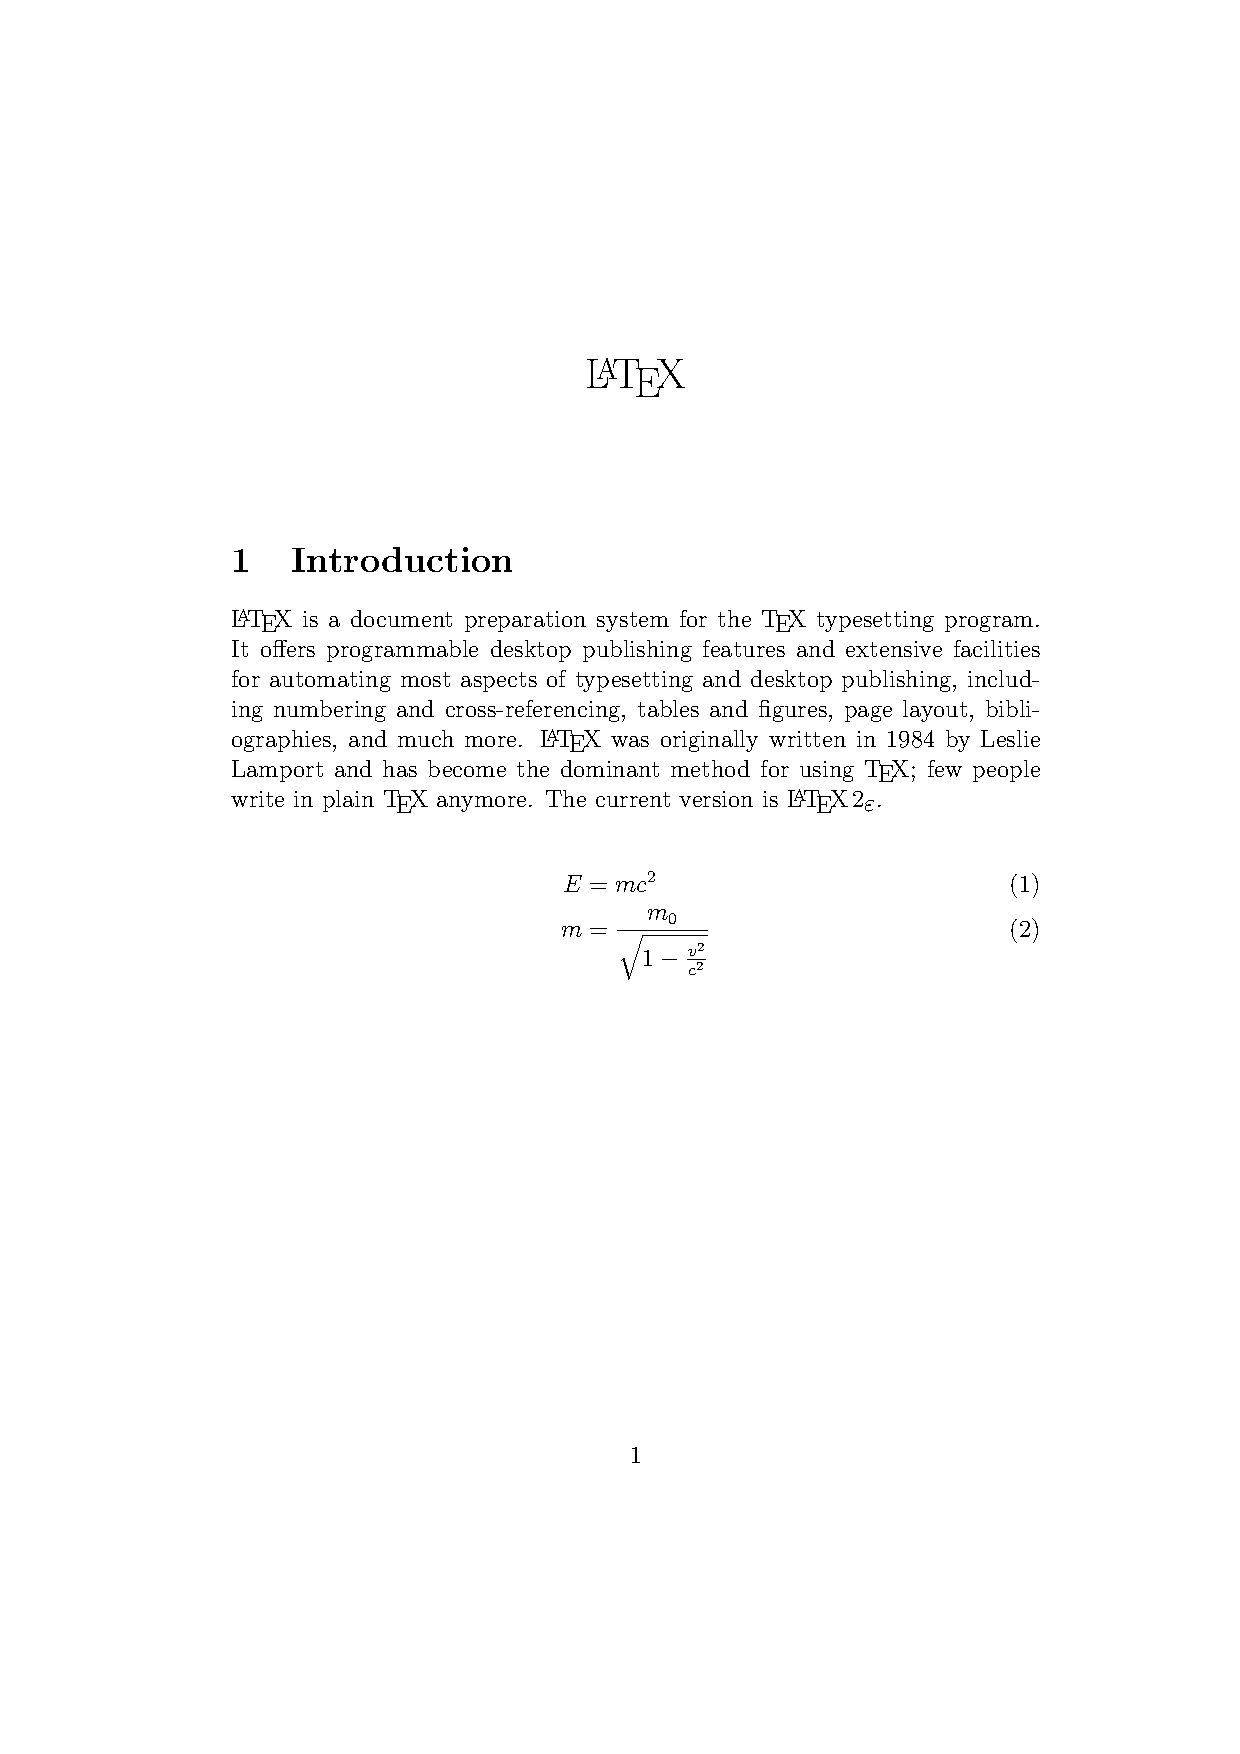
\includegraphics[trim = 33mm 127mm 33mm 59mm, clip, width=\textwidth]{figures/example_article.pdf}
  \end{framed}
  \end{minipage}
  }
}

\begin{frame}[fragile]
  \frametitle{Spaces}
{\small
\begin{verbatim}You can use LaTeX to typeset regular text.  In LaTeX, using
extra     spaces       or      a newline   doesn't matter.

However, using two newlines in a row results in a new
paragraph.\end{verbatim}
}
  \begin{minipage}{\textwidth} 
  %\begin{framed}
    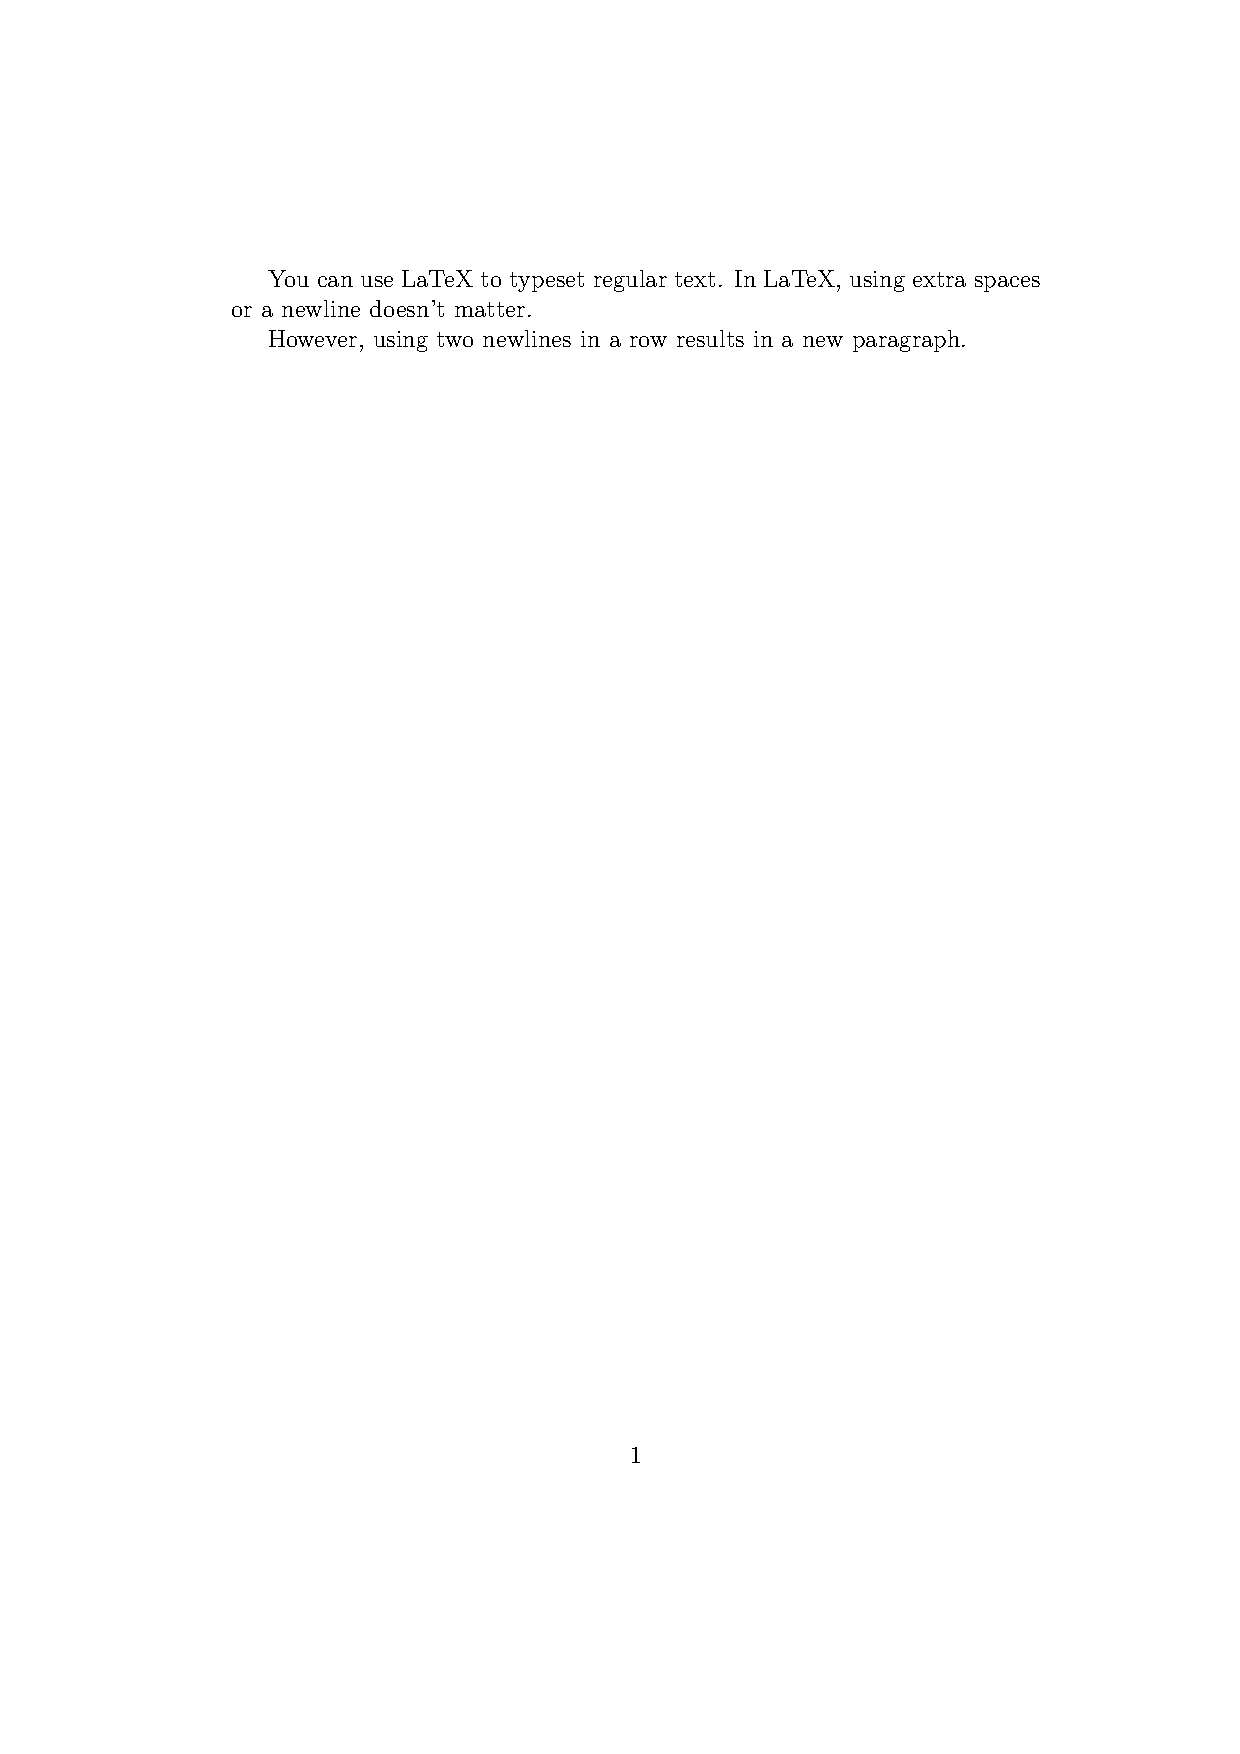
\includegraphics[trim = 33mm 230mm 33mm 40mm, clip, width=\textwidth]{figures/example_spacing.pdf}
  %\end{framed}
  \end{minipage}
\end{frame}

\begin{frame}[fragile]
  \frametitle{Control Sequences}
  \begin{itemize}
    \item \LaTeX{} uses control sequences to achieve special functionality
    \item Control sequences start with a backslash \verb|\|
  \end{itemize}
  \small
  \begin{table}
  \begin{tabular}{l l}
    \verb|\documentclass[12pt]{article}| & describes appearance of document \\
     & (similar to CSS) \\
    \verb|\begin{document}| & begins document environment \\
    \verb|\section{Section Title}| & starts a new section \\
    \verb|\subsection{Subsection Title}| & starts a new subsection \\
    \verb|\LaTeX{}| & displays \LaTeX{} \\
    \verb|\end{document}| & ends document environment
  \end{tabular}
  \end{table}
\end{frame}

\begin{frame}[fragile]
  \frametitle{Math Mode}
  \begin{itemize}
    \item Text between dollar signs \verb|$...$| will use math mode
    \item Many control sequences only work in math mode
    \item Can use \verb|^| for superscripts and \verb|_| for subscripts
  \end{itemize}
  \begin{table}
  \begin{tabular}{l l}
    \verb|$y = 3x - 4$| & $\rightarrow \quad y = 3x - 4$ \\
    \verb|$\theta \Theta \omega \Omega$| & $\rightarrow \quad \theta \Theta \omega \Omega$\\
    \verb|$\sqrt{x} = x^{1/2}$| & $\rightarrow \quad \sqrt{x} = x^{1/2}$\\
    \verb|$\min \{ x_1, x_2, x_3 \}$| & $\rightarrow \quad \min \{ x_1, x_2, x_3 \}$
  \end{tabular}
  \end{table}
\end{frame}

\begin{frame}[fragile]
  \frametitle{Displayed Math}
  \begin{itemize}
    \item Example: {\small \verb|f(x) = \sum_{i=1}^{\infty} \frac{1}{g_i(x)}|}
    \item Use dollar signs \verb|$...$| for inline math
      \begin{itemize} \item The equation $f(x) = \sum_{i=1}^{\infty} \frac{1}{g_i(x)}$ is displayed inline \end{itemize}
    \item Use escaped brackets \verb|\[...\]| to display math on its own line
      \[ f(x) = \sum_{i=1}^{\infty} \frac{1}{g_i(x)} \]
    \item Use \verb|\begin{equation}...\end{equation}| for automatically numbered equations
      \begin{equation} f(x) = \sum_{i=1}^{\infty} \frac{1}{g_i(x)} \end{equation}
  \end{itemize}
\end{frame}

\begin{frame}
  \frametitle{Exercise 2: Definition of Derivative}
  \begin{itemize}
    \item Produce the following equation in \LaTeX{}:
    \[ \frac{\mathrm{d}f(x)}{\mathrm{d}x} = \lim_{\delta \to 0} \frac{f(x + \delta) - f(x)}{\delta} \]
    \item Helpful sites:
      \begin{itemize}
        \item en.wikibooks.org/wiki/LaTeX/Mathematics
        \item ftp.ams.org/pub/tex/doc/amsmath/short-math-guide.pdf
      \end{itemize}
  \end{itemize}
\end{frame}

\begin{frame}[fragile]
  \frametitle{Exercise 2: Definition of Derivative (Solution)}
  \begin{itemize}
    \item Produce the following equation in \LaTeX{}:
    \[ \frac{\mathrm{d}f(x)}{\mathrm{d}x} = \lim_{\delta \to 0} \frac{f(x + \delta) - f(x)}{\delta} \]
    \item Solution:
  \end{itemize}
  {\small \begin{verbatim}\[
  \frac{\mathrm{d}f(x)}{\mathrm{d}x}
  = \lim_{\delta \to 0} \frac{f(x + \delta) - f(x)}{\delta}
\]\end{verbatim}}
  \begin{itemize}
    \item Do the $\mathrm{d}$s in your solution look different?
      \begin{itemize} \item \verb|\mathrm| displays upright characters in math mode \end{itemize}
  \end{itemize}
\end{frame}

\begin{frame}[fragile]
  \frametitle{Array-Like Environments}
  \begin{itemize}
    \item Use \verb|array| environment or one of the matrix environments to make table of information
    \item Matrix environments include delimiters for convenience
    \begin{itemize}
      \item \verb|pmatrix| $()$, \verb|bmatrix| $[]$, \verb|Bmatrix| $\{\}$,
      \verb|vmatrix| $| |$, \verb|Vmatrix| $\| \|$
    \end{itemize}
    \item Columns separated with \verb|&|, rows separated with \verb|\\|
%    \item Column alignment specified at start using \verb|l| for left, \verb|c| for center
%      and \verb|r| for right
%   \begin{itemize}\item Example: \verb|{ccc}| means use three centered columns\end{itemize}
  \end{itemize}

  \begin{minipage}{.47\textwidth}
  \begin{framed}
    \begin{verbatim}A = \begin{pmatrix}
      2  & -1 & 0  \\
      -1 & 2  & -1 \\
      0  & -1 & 2
    \end{pmatrix}\end{verbatim}
  \end{framed}
  \end{minipage}
  $\rightarrow$
  \begin{minipage}{.43\textwidth} 
  \begin{framed}
    \[
%      A = \left( \begin{array}{ccc}
%      2 & -1 & 0 \\
%      -1 & 2 & -1 \\
%      0 & -1 & 2 \end{array} \right)
A = \begin{pmatrix}
      2  & -1 & 0  \\
      -1 & 2  & -1 \\
      0  & -1 & 2
    \end{pmatrix}
    \]
  \end{framed}
  \end{minipage}
\end{frame}

\begin{frame}[fragile]
  \frametitle{Align Environment}
  \begin{itemize}
    \item Use \verb|align| environment to line up multiple equations
    \item Left and right sides of equation separated with \verb|&|
    \item Equations separated with \verb|\\|
    \item Using \verb|align*| instead of \verb|align| will suppress equation numbers
  \end{itemize}
  \begin{minipage}{.52\textwidth}
  \begin{framed}
    \begin{verbatim}\begin{align}
  x & = \cos(\theta(t)) \\
  y & = \sin(\theta(t)) \\
  \theta(t) &
     = \omega t + \phi
\end{align}\end{verbatim}
  \end{framed}
  \end{minipage}
  $\rightarrow$
  \begin{minipage}{.41\textwidth} 
  \begin{framed}
    \begin{align}
      x & = \cos(\theta(t)) \\
      y & = \sin(\theta(t)) \\
     \theta(t) & = \omega t + \phi
    \end{align}
  \end{framed}
  \end{minipage}
\end{frame}

\begin{frame}[fragile]
  \frametitle{Resizing Delimiters}
  \begin{itemize}
    \item The \verb|\left|, \verb|\right|, and \verb|\middle| commands are used to automatically resize
      delimiters like parenthesis based on content
    \item Period \verb|.| denotes an omitted left or right delimiter
    \item The \verb|\big|, \verb|\Big|, \verb|\bigg|, and \verb|\Bigg| commands can be used to manually resize delimiters
  \end{itemize}
  \begin{table}
  \small
  \begin{tabular}{l l}
    \verb|$\left(\frac{x^2}{y+x}\right)^2$| & $\rightarrow \quad$ \begin{minipage}{.3\textwidth} \[ \left(\frac{x^2}{y + x}\right)^2 \]\end{minipage} \\
    \begin{minipage}{.6\textwidth}\begin{verbatim}$P\left(X=1 \middle|
  \frac{X}{Y} \geq 2 \right)$\end{verbatim}\end{minipage} & $\rightarrow \quad$ \begin{minipage}{.3\textwidth} \[ P\left(X=1 \middle|\frac{X}{Y} \geq 2\right) \]\end{minipage} \\
    \verb!$\left.2x-\frac{2}{x^3}\right|_0^1$! & $\rightarrow \quad$ \begin{minipage}{.3\textwidth}\[ \left.2x - \frac{2}{x^3}\right|_0^1\] \end{minipage} \\
    \verb|$( \big( \Big( \bigg( \Bigg($| & $\rightarrow \quad$ \begin{minipage}{.3\textwidth}\[ ( \big( \Big( \bigg( \Bigg( \] \end{minipage} 
  \end{tabular}
  \end{table}
\end{frame}

\begin{frame}[fragile]
  \frametitle{Math Accents}
  \begin{itemize} \item Special accents over variables/expressions may be used in math mode \end{itemize}
  \begin{table}
  \begin{tabular}{l l l l}
    \verb|$\bar{x}$| & $\rightarrow \quad \bar{x}$ &
    \qquad \qquad \verb|$\vec{x}$| & $\rightarrow \quad \vec{x}$ \\
    \verb|$\dot{x}$| & $\rightarrow \quad \dot{x}$ &
    \qquad \qquad \verb|$\hat{x}$| & $\rightarrow \quad \hat{x}$ \\
    \verb|$\ddot{x}$| & $\rightarrow \quad \ddot{x}$ &
    \qquad \qquad \verb|$\tilde{x}$| & $\rightarrow \quad \tilde{x}$ \\
    \verb|$\acute{x}$| & $\rightarrow \quad \acute{x}$ &
    \qquad \qquad \verb|$\grave{x}$| & $\rightarrow \quad \grave{x}$
  \end{tabular}
  \end{table}
\end{frame}

\begin{frame}
  \frametitle{Exercise 3: Matrices}
  \begin{itemize}
    \item Produce the following equations in \LaTeX{}:
      \begin{align*}
        \begin{vmatrix}a & b \\ c & d\end{vmatrix} & = ad - bc \\
        \vec{x} & = \begin{pmatrix}x_1 & x_2 & \cdots & x_n\end{pmatrix}^\mathsf{T}
      \end{align*}
    \item Helpful sites:
      \begin{itemize}
        \item en.wikibooks.org/wiki/LaTeX/Mathematics
        \item ftp.ams.org/pub/tex/doc/amsmath/short-math-guide.pdf
      \end{itemize}
  \end{itemize}
\end{frame}

\begin{frame}[fragile]
  \frametitle{Exercise 3: Matrices (Solution)}
  \begin{itemize}
    \item Produce the following equations in \LaTeX{}:
      \begin{align*}
        \begin{vmatrix}a & b \\ c & d\end{vmatrix} & = ad - bc \\
        \vec{x} & = \begin{pmatrix}x_1 & x_2 & \cdots & x_n\end{pmatrix}^\mathsf{T}
      \end{align*}
    \item Solution:
  \end{itemize}
  {\small \begin{verbatim}\begin{align*}
  \begin{vmatrix} a & b \\ c & d \end{vmatrix} & = ad - bc \\
  \vec{x} & = \begin{pmatrix}
    x_1 & x_2 & \cdots & x_n
    \end{pmatrix}^\mathsf{T}
\end{align*}\end{verbatim}}
  \begin{itemize}
    \item There is some variation and debate about how best to typeset certain things
      (e.g.\ matrix transpose operator)
  \end{itemize}
\end{frame}

\end{document}

\end{document}
